\documentclass[compress]{beamer}

\usepackage{multicol}
\usepackage{tikz}
\usetikzlibrary{shapes}
\usetikzlibrary{arrows}
\usetikzlibrary{patterns}

\usetheme{Szeged}
%\usetheme{PaloAlto}
\usecolortheme{beaver}

\title[Department of Nuclear Engineering and Engineering Physics]{Selective Spatial-Temporal Nonlinear Refinement For
Thermal-Hydraulic Safety Analysis Codes}
\author[Lloyd]{Lewis John Lloyd}
\institute[University of Wisconsin - Madison]
{
  Department of Nuclear Engineering and Engineering Physics \\
  University of Wisconsin - Madison
}
\date[Prelim Defense 2012]{Preliminary Defense, 2012}
\subject{Nuclear Engineering}

\setbeamertemplate{navigation symbols}{}

\newcommand{\origaddtocontents}{\addtocontents}
\newcommand{\dontaddtocontents}{}

\begin{document}
%------------------------------------------------------------------------------
%------------------------------------------------------------------------------

%\AtBeginSubsection[]
%{
%\begin{frame}
%\tableofcontents[subsectionstyle=show/shaded/hide,sectionstyle=show/shaded]
%\end{frame}
%}

%------------------------------------------------------------------------------
%------------------------------------------------------------------------------
\frame{\titlepage}
%------------------------------------------------
%------------------------------------------------
\begin{frame}
\begin{multicols}{2}
\tableofcontents
\end{multicols}
\end{frame}
%------------------------------------------------------------------------------
%------------------------------------------------------------------------------
\section[Background and Introduction]{Background and Introduction}
%------------------------------------------------
%------------------------------------------------
\begin{frame}
\frametitle{Introduction}

\begin{itemize}
\item{test1}
\item{test2}
\end{itemize}

\end{frame}
%------------------------------------------------------------------------------
%------------------------------------------------------------------------------
\subsection[Geometry]{Geometry of Interest}
%------------------------------------------------
%------------------------------------------------
\begin{frame}
\frametitle{Geometric Components}
\begin{columns}
\column{0.5\textwidth}

\begin{itemize}
\item{Sections}
\item{Channels}
\item{Gaps}
\item{Solid Structures}
\end{itemize}

\column{0.5\textwidth}
\begin{figure}[t]
\centering
\resizebox{!}{0.7\textheight}{
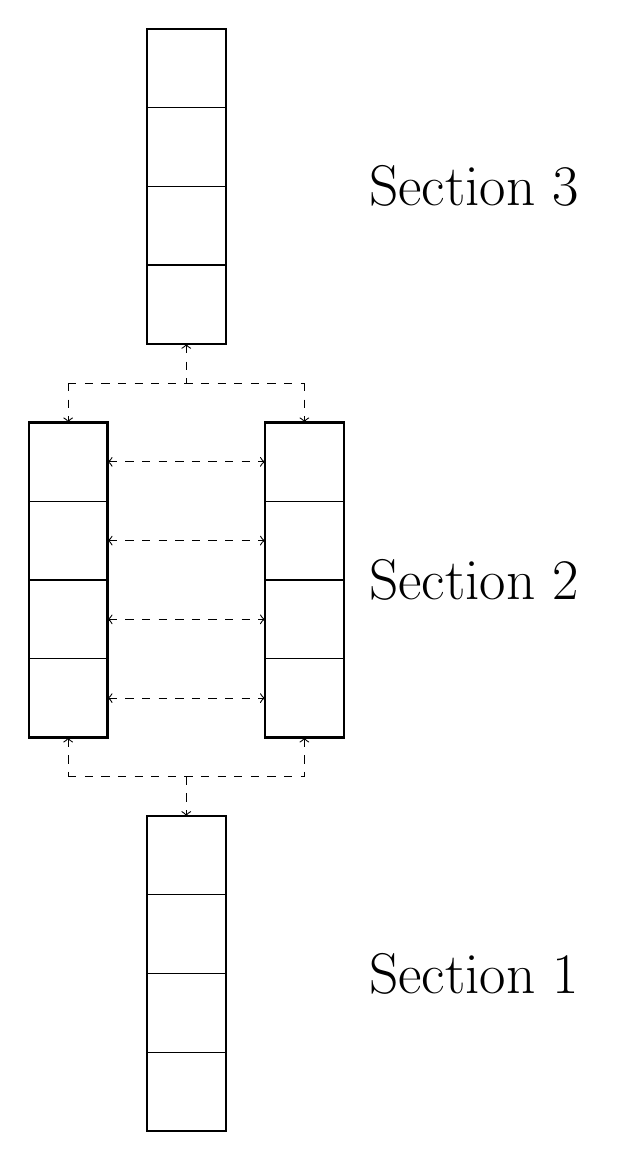
\begin{tikzpicture}
\draw [thick] (-2,-2) rectangle (-1,2);
\draw [thick] (1,-2) rectangle (2,2);
\draw [thick] (-0.5,3) rectangle (0.5,7);
\draw [thick] (-0.5,-7) rectangle (0.5,-3);
\draw [dashed] (-1.5,2.5) -- (1.5,2.5);
\draw [dashed](-1.5,-2.5) -- (1.5,-2.5);
\draw [dashed,<-] (0,3) -- (0,2.5);
\draw [dashed,->] (-1.5,2.5) -- (-1.5,2);
\draw [dashed,->] (1.5,2.5) -- (1.5,2);
\draw [dashed,->] (0,-2.5) -- (0,-3);
\draw [dashed,<-] (-1.5,-2) -- (-1.5,-2.5);
\draw [dashed,<-] (1.5,-2) -- (1.5,-2.5);
\foreach \y in {-1.5, -0.5, 0.5, 1.5}
	\draw [dashed, <->] (-1,\y) -- (1,\y);
\foreach \y in {-6,-5,-4,4,5,6}
	\draw (-0.5,\y) -- (0.5,\y);
\foreach \y in {-1,0,1}
	\draw (-2,\y) -- (-1,\y);
\foreach \y in {-1,0,1}
	\draw (1,\y) -- (2,\y);
\foreach \y/\ytext in {-5/ 1,0/ 2,5/ 3}
	\draw (2.2,\y) node [anchor=west] {\huge Section $\ytext$};
\end{tikzpicture}
}
\end{figure}

\end{columns}

\end{frame}
%------------------------------------------------
%------------------------------------------------

\begin{frame}
\frametitle{Staggered Grid}

\begin{columns}
\column{0.5\textwidth}
I will talk about staggered grids?
I may talk about staggered grids.
Who knows.
\begin{itemize}
\item{Continuity Volumes}
\item{Momentum Volumes}
\end{itemize}
\column{0.5\textwidth}
\begin{figure}
\centering
\resizebox{\textwidth}{!}{
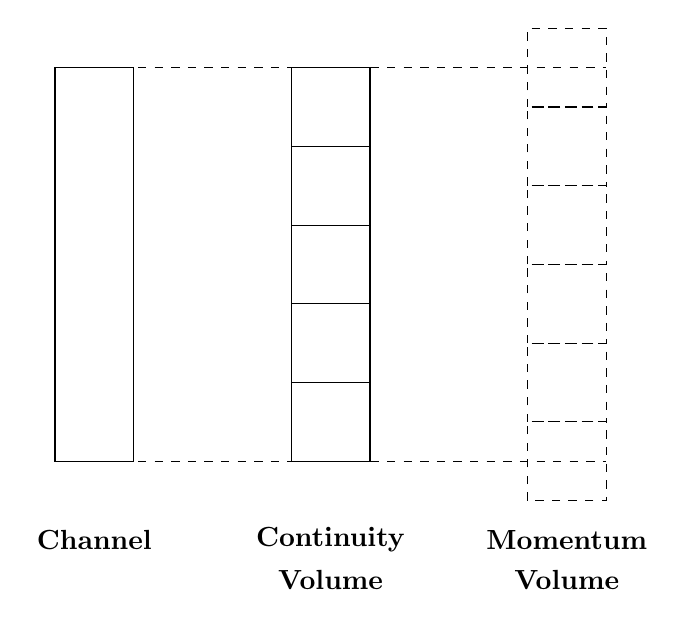
\begin{tikzpicture}
\draw (-3,0) rectangle +(1,5);
\draw (0,0) rectangle +(1,1) (0,1) rectangle +(1,1) (0, 2) rectangle +(1,1) (0,3) rectangle +(1,1) (0,4) rectangle +(1,1);
\draw[dashed] (3,-0.5) rectangle +(1,1) (3,0.5) rectangle +(1,1) (3,1.5) rectangle +(1,1) (3, 2.5) rectangle +(1,1) (3,3.5) rectangle +(1,1) (3,3.5) rectangle +(1,1) (3, 4.5) rectangle +(1,1) ;
\draw[dashed] (-3,0) -- (4,0);
\draw[dashed] (-3,5) -- (4,5);
\draw (-2.5,-1) node {\textbf{Channel}};
\draw (0.5,-1) node {\textbf{Continuity}};
\draw (0.5,-1.5) node {\textbf{Volume}};
\draw (3.5,-1) node {\textbf{Momentum}};
\draw (3.5,-1.5) node {\textbf{Volume}};
\end{tikzpicture}
}
\end{figure}
\end{columns}

\end{frame}
%------------------------------------------------------------------------------
%------------------------------------------------------------------------------
\subsection[Two-Phase Flow]{Two-Phase Flow}
%------------------------------------------------
%------------------------------------------------
\begin{frame}
\frametitle{Two-Phase Flow}

\begin{itemize}
\item{Background}
\item{Assumptions}
\item{Equations}
\end{itemize}

\end{frame}
%------------------------------------------------
%------------------------------------------------
\begin{frame}
\frametitle{Conservation of Mass}

Yay for more math.

\end{frame}
%------------------------------------------------
%------------------------------------------------
\begin{frame}
\frametitle{Conservation of Momentum}

Yay for more math.

\end{frame}
%------------------------------------------------
%------------------------------------------------
\begin{frame}
\frametitle{Conservation of Energy}

Yay for more math.

\end{frame}
%------------------------------------------------------------------------------
%------------------------------------------------------------------------------
\subsection[Numeric Approximation]{Numerical Approximations}
%------------------------------------------------
%------------------------------------------------
\begin{frame}
\frametitle{Spatial Approximations}

\begin{itemize}
\item{1st Order Upwind}
\item{Continuity Volume}
\item{Momentum Volume}
\end{itemize}

\end{frame}
%------------------------------------------------
%------------------------------------------------
\begin{frame}
\frametitle{Temporal Approximations}

\begin{itemize}
\item{Single-Step}
\item{Single-Stage}
\item{Multi-Stage}
\end{itemize}

\end{frame}
%------------------------------------------------
%------------------------------------------------
\begin{frame}
\frametitle{Nonlinear Equations}

\begin{itemize}
\item{System of nonlinear Equations.}
\item{Residuals.}
\end{itemize}

\end{frame}
%------------------------------------------------------------------------------
%------------------------------------------------------------------------------
\subsection[Solution Methods]{Solution Methods}
%------------------------------------------------
%------------------------------------------------
\begin{frame}
\frametitle{Fully-Explicit Method}

Here I talk about the Fully-Explicit Method

\end{frame}
%------------------------------------------------
%------------------------------------------------
\begin{frame}
\frametitle{Fully-Implicit Method}

Here I talk about the fully-implicit method.

\end{frame}
%------------------------------------------------
%------------------------------------------------
\begin{frame}
\frametitle{Semi-Implicit Method Overview}

Semi-Implicit method.

\end{frame}
%------------------------------------------------
%------------------------------------------------
\begin{frame}
\frametitle{Semi-Implicit Method Solver}

Details

\end{frame}
%------------------------------------------------
%------------------------------------------------
\begin{frame}
\frametitle{Semi-Implicit Method Solver}

More Details

\end{frame}
%------------------------------------------------
%------------------------------------------------
\begin{frame}
\frametitle{Stability-Enhancing Two-Step Method}

Sets.

\end{frame}
%------------------------------------------------
%------------------------------------------------
\begin{frame}
\frametitle{Nearly-Implicit Method}

Nearly Implicit

\end{frame}
%------------------------------------------------------------------------------
%------------------------------------------------------------------------------
\subsection[Algorithmic Concerns]{Algorithmic Concerns}
%------------------------------------------------
%------------------------------------------------
\begin{frame}
\frametitle{Phase Transition}

Phases are transitioned.

\end{frame}
%------------------------------------------------
%------------------------------------------------
\begin{frame}
\frametitle{Time Step Failure Mitigation}

Time step failures are mitigated.

\end{frame}
%------------------------------------------------
%------------------------------------------------
\begin{frame}
\frametitle{Time-step selection}

Time step are selected.

\end{frame}
%------------------------------------------------------------------------------
%------------------------------------------------------------------------------
\subsection[Domain Coupling]{Domain Coupling}
%------------------------------------------------
%------------------------------------------------
\begin{frame}
\frametitle{Code Coupling}

Codes are coupled.

Figure of two codes talking.

\end{frame}
%------------------------------------------------
%------------------------------------------------
\begin{frame}
\frametitle{RELAP5-3D coupling}

Pressure Updates
Codes are coupled.

Figure of two codes talking.

\end{frame}
%------------------------------------------------
%------------------------------------------------
\begin{frame}
\frametitle{Domain Decomposition.}

Figure of one domain with two sub components.
Talk about additive Schwarz methods.
Talk about multiplicative Schwarz methods.

\end{frame}
%------------------------------------------------------------------------------
%------------------------------------------------------------------------------
\subsection[Research Objectives]{Research Objectives}
%------------------------------------------------
%------------------------------------------------
\begin{frame}
\frametitle{Research Objectives}

I am the objective.
Here is where I talk about stuff.
Fun stuff.

\end{frame}
%------------------------------------------------------------------------------
%------------------------------------------------------------------------------
\section[Preliminary Work]{Preliminary Work}
%------------------------------------------------
%------------------------------------------------
\subsection[COBRA]{Nonlinear COBRA}
%------------------------------------------------
%------------------------------------------------
\begin{frame}
\frametitle{Work on COBRA.}

Issues.
Coding Details
Nonlinear Solver


\end{frame}
%------------------------------------------------
%------------------------------------------------
\begin{frame}
\frametitle{Linesearch Algorithm}

Issues.
Coding Details
Nonlinear Solver


\end{frame}
%------------------------------------------------------------------------------
%------------------------------------------------------------------------------
\subsection[Scaling]{Operator Based Scaling}
%------------------------------------------------
%------------------------------------------------
\begin{frame}
\frametitle{Scaling One}

Stuff gets scaled.

\end{frame}
%------------------------------------------------
%------------------------------------------------
\begin{frame}
\frametitle{Scaling Two}

Stuff gets scaled again.

\end{frame}
%------------------------------------------------------------------------------
%------------------------------------------------------------------------------
\subsection[Convergence]{Temporal Convergence}
%------------------------------------------------
%------------------------------------------------
\begin{frame}
\frametitle{Time is Converged.}

Convergence occurs.

\end{frame}
%------------------------------------------------------------------------------
%------------------------------------------------------------------------------
\subsection[Experiments]{Numerical Experiments}
%------------------------------------------------
%------------------------------------------------
\begin{frame}
\frametitle{Purpose}

I am the purpose.

\end{frame}
%------------------------------------------------
%------------------------------------------------
\begin{frame}
\frametitle{Geometry}

Geometry goes here.

\end{frame}
%------------------------------------------------
%------------------------------------------------
\begin{frame}
\frametitle{Initial and Boundary Conditions}

Here are the conditions.

\end{frame}
%------------------------------------------------
%------------------------------------------------
\begin{frame}
\frametitle{Procedure}

Procedures are good.

\end{frame}
%------------------------------------------------
%------------------------------------------------
\begin{frame}
\frametitle{Results 1}

Stuff

\end{frame}
%------------------------------------------------
%------------------------------------------------
\begin{frame}
\frametitle{Results 2}

Results are good.

\end{frame}
%------------------------------------------------
%------------------------------------------------
\begin{frame}
\frametitle{Results 3}

Results are better.

\end{frame}
%------------------------------------------------
%------------------------------------------------
\begin{frame}
\frametitle{Results 4}

Results are best.

\end{frame}
%------------------------------------------------------------------------------
%------------------------------------------------------------------------------
\subsection[Review]{Review}
%------------------------------------------------
%------------------------------------------------
\begin{frame}
\frametitle{Review of Work.}

Here I review.

\end{frame}
%------------------------------------------------
%------------------------------------------------
\begin{frame}
\frametitle{Review 2.}

Review part 2.

\end{frame}
%------------------------------------------------------------------------------
%------------------------------------------------------------------------------
\section[Proposed Work]{Proposed Work}
%------------------------------------------------
%------------------------------------------------
\begin{frame}
\frametitle{Here is a time line overview.}

Timeline goes here.

\end{frame}
%------------------------------------------------------------------------------
%------------------------------------------------------------------------------
\subsection[Scaling]{Scaling Work}
%------------------------------------------------
%------------------------------------------------
\begin{frame}
\frametitle{Scaling Work.}

Scaling stuff.

\end{frame}
%------------------------------------------------------------------------------
%------------------------------------------------------------------------------
\subsection[Domain Decomposition]{Domain Decomposition}
%------------------------------------------------
%------------------------------------------------
\begin{frame}
\frametitle{Domains get decomposed.}

More decomposition.

\end{frame}
%------------------------------------------------------------------------------
%------------------------------------------------------------------------------
\subsection[Testing]{Testing and Benchmarking}
%------------------------------------------------
%------------------------------------------------
\begin{frame}
\frametitle{Testing.}

Here there be testing.

\end{frame}
%------------------------------------------------------------------------------
%------------------------------------------------------------------------------
\subsection[Time Line]{Time Line}
%------------------------------------------------
%------------------------------------------------
\begin{frame}
\frametitle{Time Line Again.}

I am stuff.

\end{frame}
%------------------------------------------------------------------------------
%------------------------------------------------------------------------------
\subsection[Possible Outcomes]{Possible Outcomes}
%------------------------------------------------
%------------------------------------------------
\begin{frame}
\frametitle{This is the fourth slide.}

I am stuff.

\end{frame}
%------------------------------------------------------------------------------
%------------------------------------------------------------------------------
\section*{}
%------------------------------------------------
%------------------------------------------------
\begin{frame}
\frametitle{Acknowledgments}

This research was performed under appointment to the Rickover Fellowship Program in Nuclear Engineering sponsored by Naval Reactors Division of the U.S. Department of Energy.

\end{frame}
%------------------------------------------------
%------------------------------------------------
\begin{frame}
\frametitle{I am another extra slide.}

I am more excess.

\end{frame}
%------------------------------------------------
%------------------------------------------------
\begin{frame}
\frametitle{I am another extra slide.}

I am more excess.

\end{frame}
%------------------------------------------------------------------------------
%------------------------------------------------------------------------------
\end{document}